\chapter{Aligning Romansh to Italian}\label{app:rm-it}

Due to the nature of my research question, I virtually ignored in the course of this work the issue of word alignments using embeddings (i.e., SimAlign) between Romansh and Italian. 
Therefore, I would like to curtly attend this issue in this appendix part.

Romansh and Italian share many similarities. 
Both of them are Romance languages and some researchers even consider Romansh to be a part of the Italian dialect continuum (see Section~\ref{sec:rhaeto-romance}). 

Since 1-to-many alignments and differing word order are more challenging to model than 1-to-1 alignments and similar or identical word order---word order or 1-to-many alignments are not modeled by IBM Model 1, but only by higher models \autocite{brown-etal-1993-mathematics}---one might expect that it should be easier to word-align languages that are more similar in structure, word order and grammar. 
That is, word-aligning Romansh to Italian should be easier than aligning Romansh to German due to the higher similarity between the former languages.
Further, when dealing with unseen languages, as in the case of Romansh, multilingual language models have been shown to favor language similarity and vocabulary overlaps \autocite{pires-etal-2019-multilingual}. 
All this gives rise to the assumption that word alignment for Romansh--Italian might perform better.

I randomly hand-picked a few examples\footnote{The only precondition was that the sentences be short; Visualization for longer sentences leaves something to be desired.} and compared SimAlign's performance on the pairs Romansh-Italian and Romansh-German in order to unempircally\footnote{Obviously, a gold standard for Romansh-Italian would be needed.} test this notion.

The plots in this part were generated using SimAlign's demo website\footnote{\url{https://simalign.cis.lmu.de}}.

\section{Examples}
Figure~\ref{fig:nov-med} is an example for a word alignment that works perfectly both with Italian and with German. 
In Figure~\ref{fig:connex}\footnote{Apologies for the somewhat unreadable edges in Romansh--German}, word alignment works well with Italian and German exactly for the same Romansh words, and it is exactly the same words where SimAlign fails: 
Romansh \emph{en quest connex} (\enquote{in this context/matter}) is not aligned correctly, neither in German nor in Italian. 
The same applies for Romansh \emph{vegn} (literally \enquote{come}, but here part of the passive construction), which is misaligned both times.
This is also the case in Figure~\ref{fig:regenza}. 
The same words are aligned correctly with German and with Italian, 
but in both cases Romansh \emph{chantun} (\enquote{canton}) remains unaligned.


\begin{figure}
	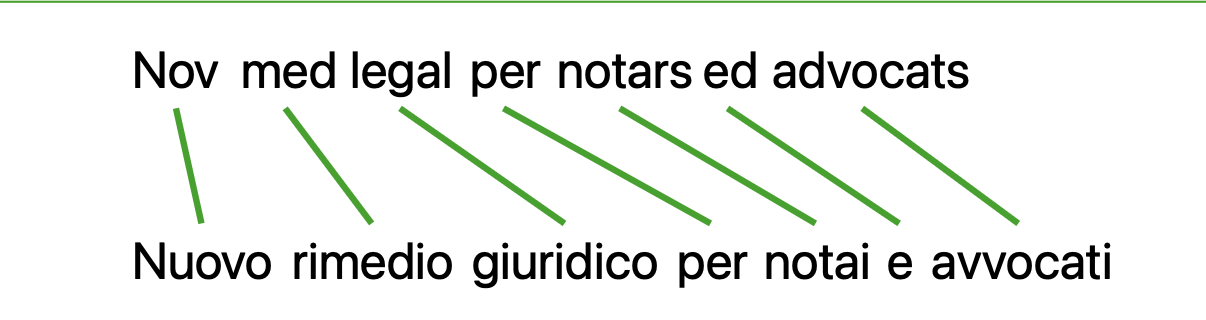
\includegraphics[width=0.9\textwidth]{graphics/alignments/it/nov-med-it.png}
	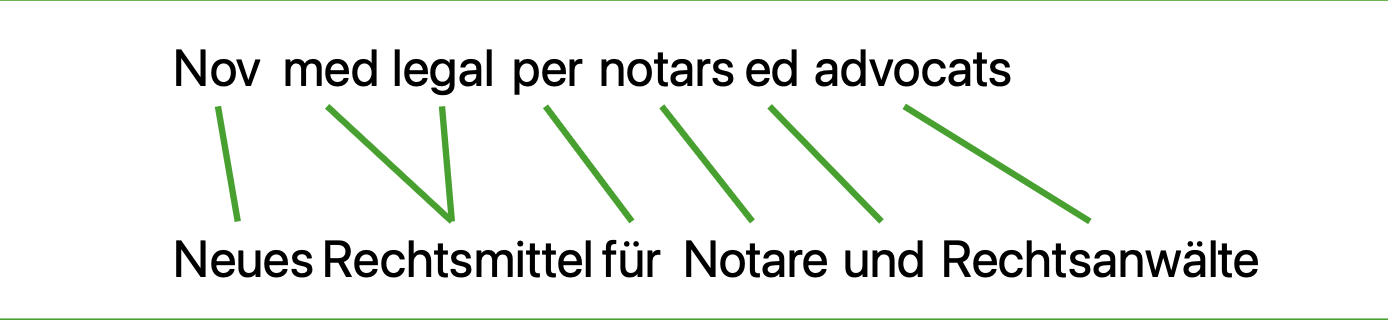
\includegraphics[width=0.9\textwidth]{graphics/alignments/it/nov-med-de.png}
	\caption{Word alignment example Romansh--Italian and Romansh--German}
	\label{fig:nov-med}
\end{figure}


\begin{figure}
	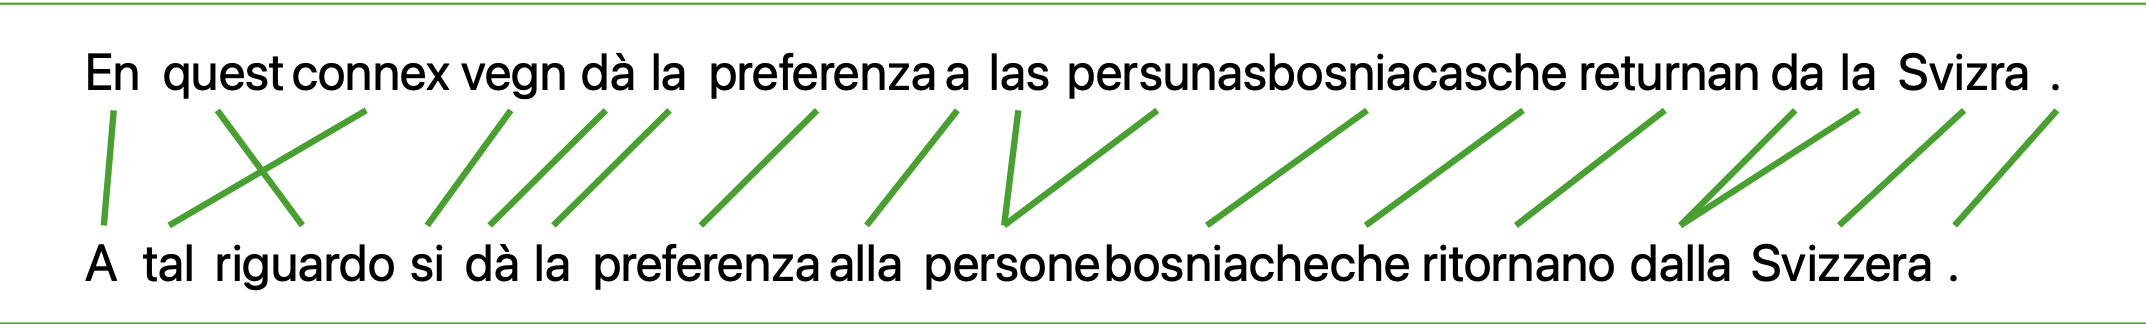
\includegraphics[width=1.1\textwidth]{graphics/alignments/it/connex-it.png}
	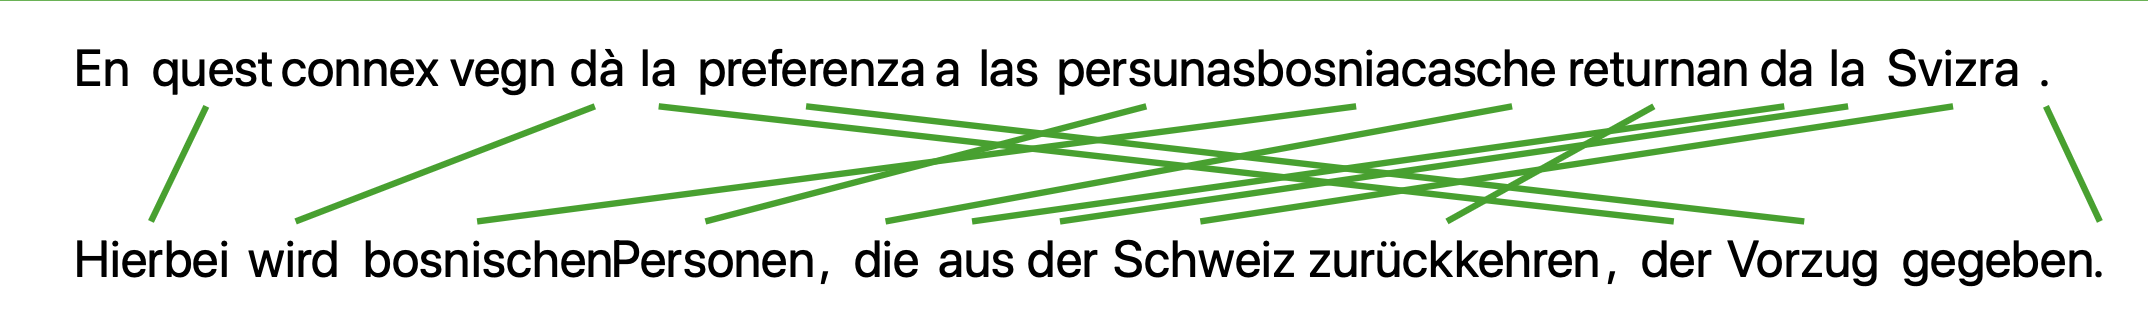
\includegraphics[width=1.1\textwidth]{graphics/alignments/it/connex-de.png}
	\caption{Word alignment example Romansh--Italian and Romansh--German}
	\label{fig:connex}
\end{figure}

\begin{figure}
	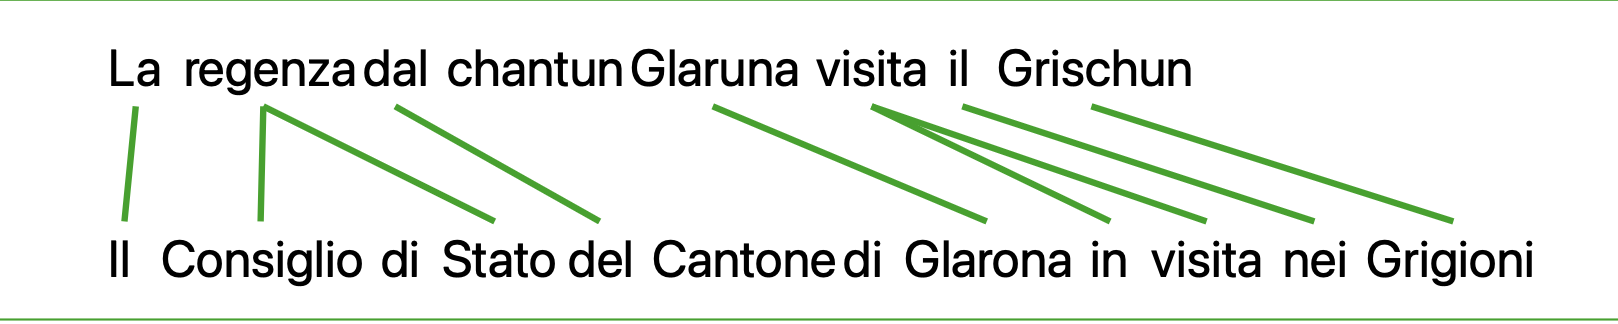
\includegraphics[width=0.9\textwidth]{graphics/alignments/it/regenza-it.png}
	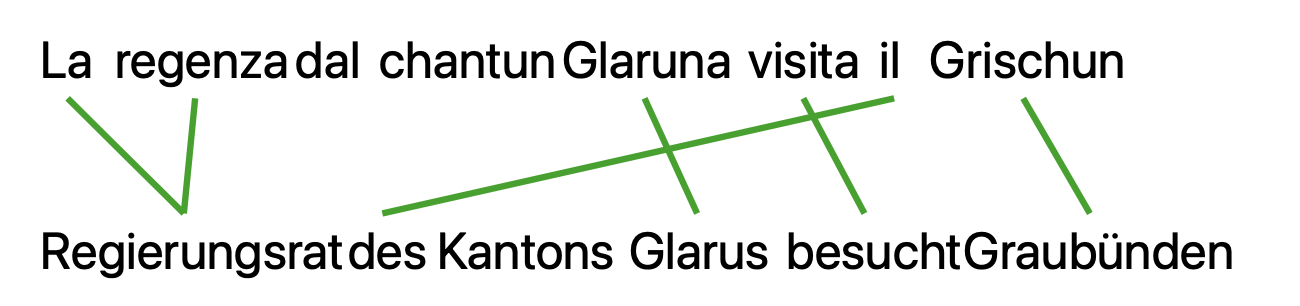
\includegraphics[width=0.9\textwidth]{graphics/alignments/it/regenza-de.png}
	\caption{Word alignment example Romansh--Italian and Romansh--German}
	\label{fig:regenza}
\end{figure}


In Figure~\ref{fig:co} word alignment with German is even better than with Italian. 
Here, every alignment is correct, whereas in the Italian example, Romansh \emph{schilar} (\enquote{tackle}) is not aligned to Italian \emph{affronatare}, which should have been the case.


\begin{figure}
	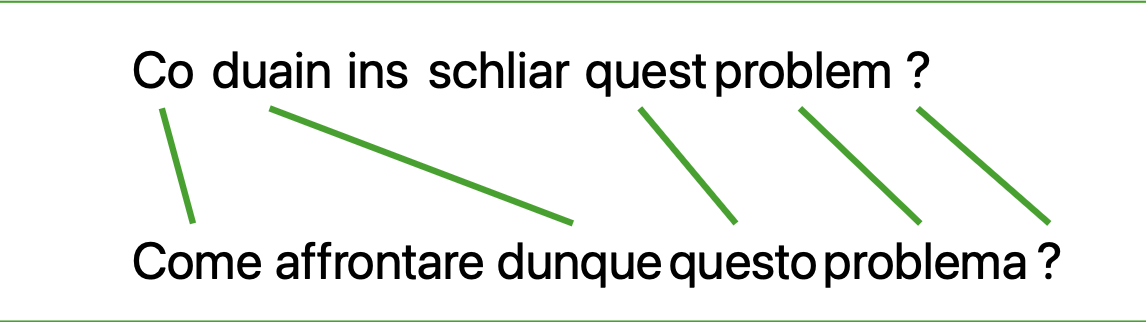
\includegraphics[width=0.9\textwidth]{graphics/alignments/it/co-it.png}
	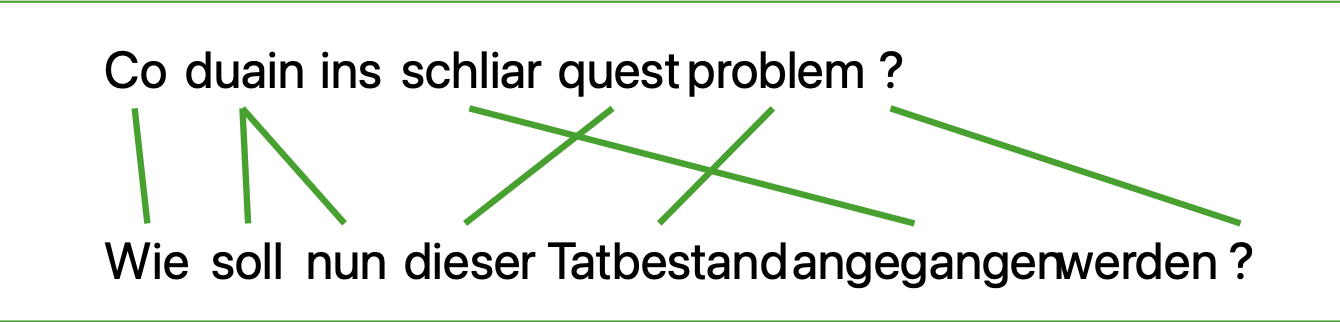
\includegraphics[width=0.9\textwidth]{graphics/alignments/it/co-de.png}
	\caption{Word alignment example Romansh--Italian and Romansh--German}
	\label{fig:co}
\end{figure}


Finally, Figure~\ref{fig:durchseuchung} is an example for many misalignments. 
In the German example, SimAlign succeeds in aligning Romansh \emph{la derasaziuna da infecziuns} to German \emph{die Durchseuchung}, but the rest of the alignments are wrong. 
The Italian example is completely misaligned.

\begin{figure}
	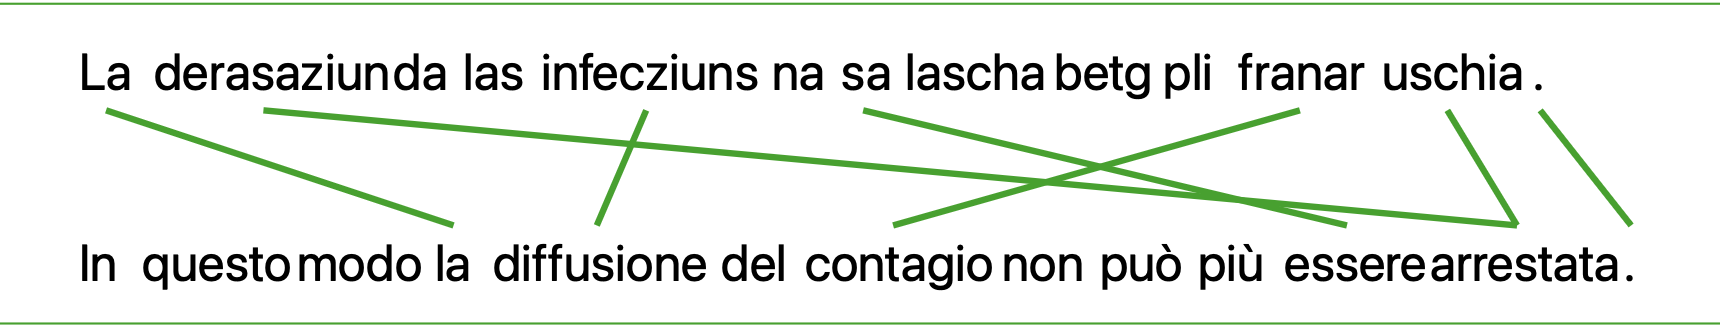
\includegraphics[width=0.9\textwidth]{graphics/alignments/it/durchseuchung-it.png}
	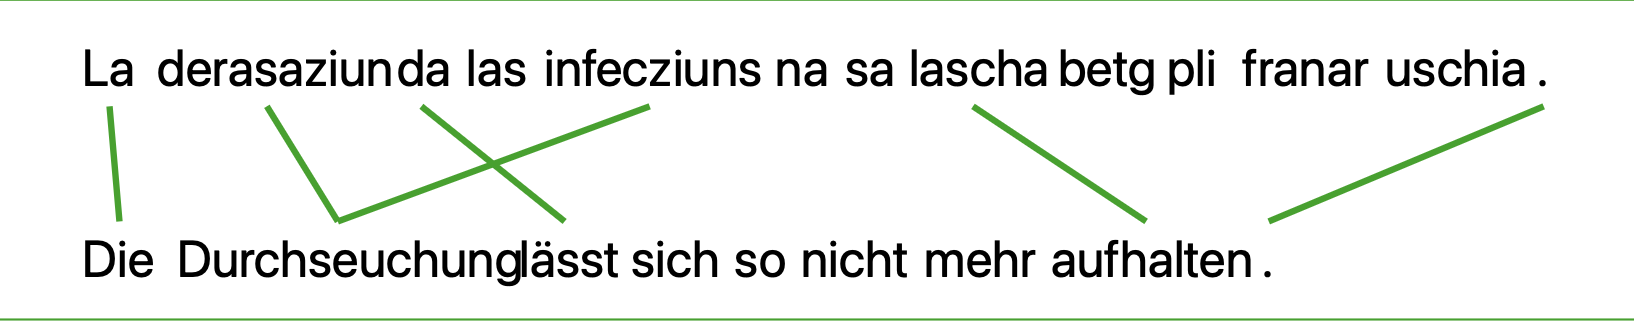
\includegraphics[width=0.9\textwidth]{graphics/alignments/it/durchseuchung-rm.png}
	\caption{Word alignment example Romansh--Italian and Romansh--German}
	\label{fig:durchseuchung}
\end{figure}

\section{Summary}
From observing these very few hand-picked cases, SimAlign doesn't seem to perform better when aligning Romansh to Italian. 
This is in spite of the higher similarity between Romansh and Italian, compared with German. 

One possible explanation for this is that what mostly influences performance is the quality of the embeddings. 
If the Romansh word is similar enough to any of the words (or subwords) in the language model, alignment will work, regardless of the target language. Take for example Figure~\ref{fig:nov-med}. 
Here, all of the Romansh words are reminiscent of other seen languages and alignment works perfectly. 
However, in the case of Figure~\ref{fig:regenza}, a suitable embedding for the Romansh word \emph{chantun} apparently cannot be looked-up, hence the word remains unaligned in both cases.


